\section{Experimentos y resultados}
\label{sec:exp}

\subsection{Configuración}
El procedimiento de evaluación cuantifica dos métricas clave de la política codiciosa ($\varepsilon=0$): la tasa de éxito en alcanzar la meta y la longitud media de la trayectoria (número de pasos). La evaluación se efectúa sobre 20 configuraciones de inicio fijas generadas de forma independiente a la muestra de entrenamiento (es decir, estados no observados previamente por el agente). Asimismo, se evalúa la desviación de costo acumulado respecto al camino óptimo global determinado mediante el algoritmo de Dijkstra.

\subsection{DQN con meta fija}
La evolución del aprendizaje de la variante DQN principal se ilustra en la Fig.~\ref{fig:curva}. El agente converge de manera estable a una \textbf{tasa de éxito del 100\,\%} (20 de 20 trayectorias de prueba resueltas). La Fig.~\ref{fig:rutas} presenta una comparación espacial de las trayectorias aprendidas por el agente en contraste con las trayectorias óptimas de Dijkstra. Evaluado sobre el conjunto completo de prueba, el agente presenta una brecha media de costo de únicamente el \textbf{3,3\,\%}, un valor notable considerando que la red neuronal opera bajo observación parcial y no posee conocimiento del mapa topográfico global.

\begin{figure}[ht]
\centering
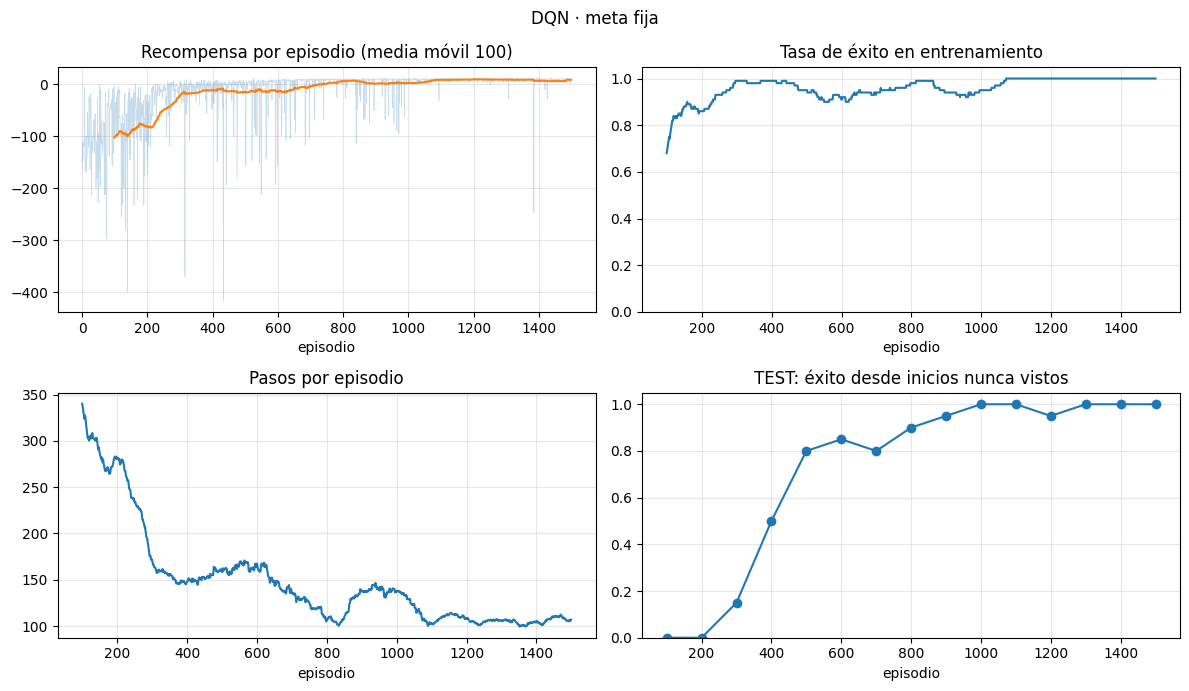
\includegraphics[width=\columnwidth]{figuras/03_curva_dqn.png}
\caption{Curva de aprendizaje de DQN con meta fija: recompensa, tasa de éxito de entrenamiento, pasos y test sobre inicios no vistos.}
\label{fig:curva}
\end{figure}

\begin{figure}[ht]
\centering
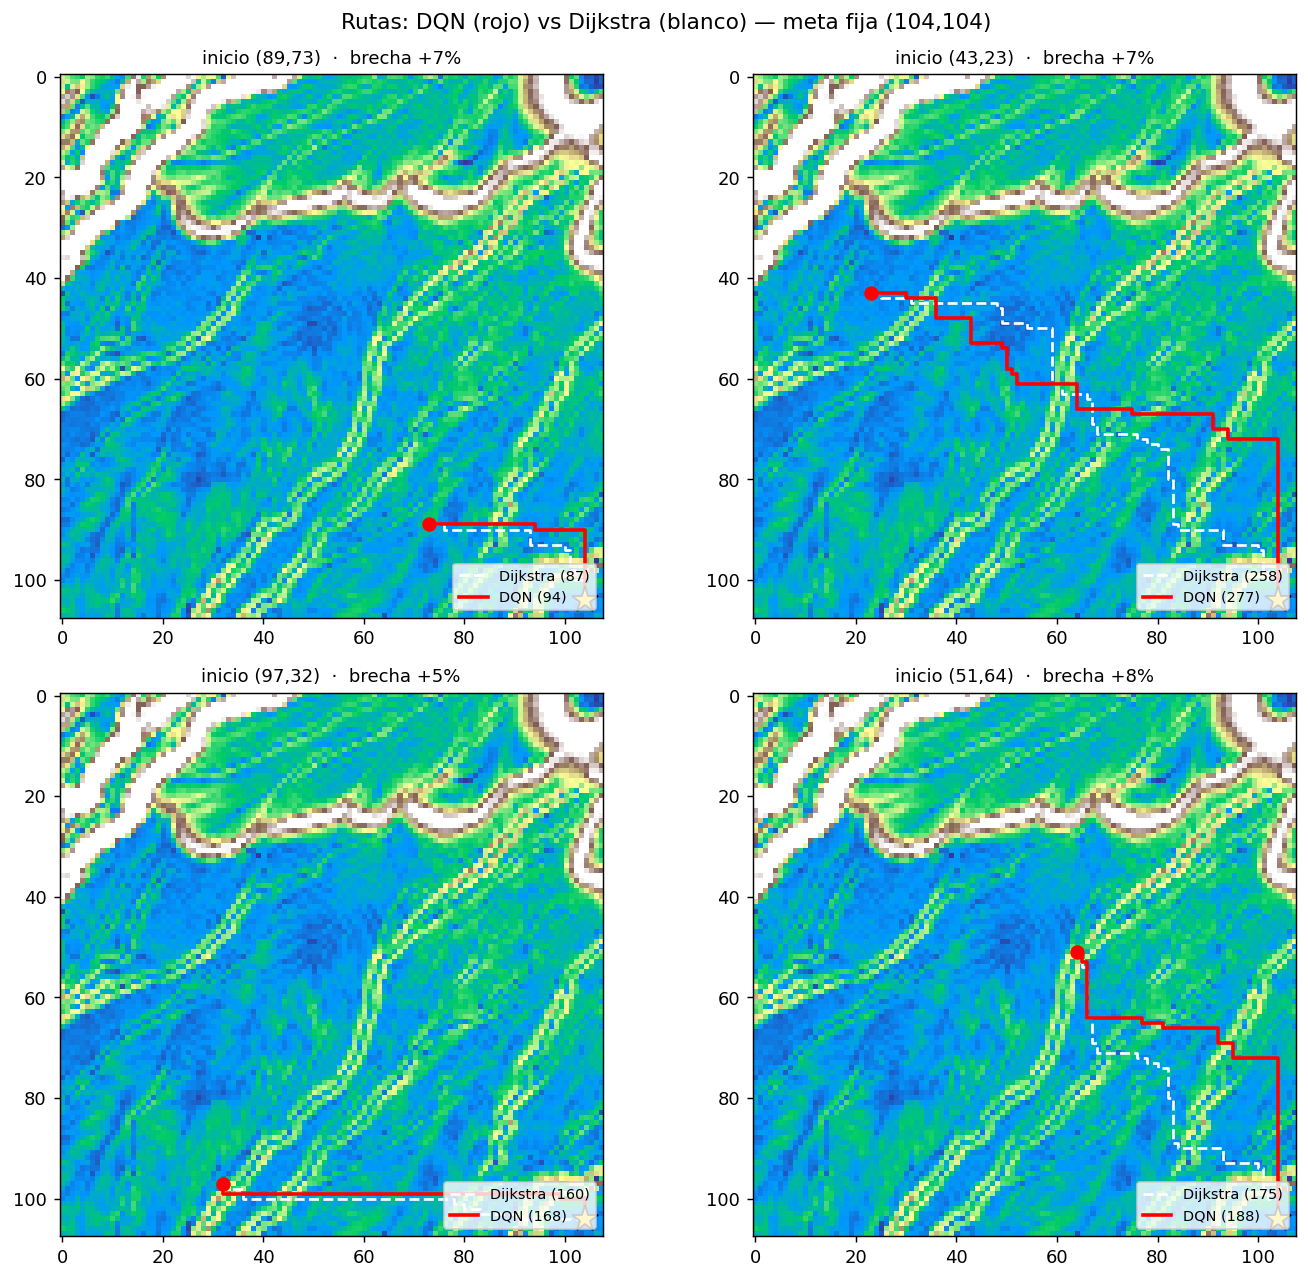
\includegraphics[width=\columnwidth]{figuras/04_rutas_dijkstra.png}
\caption{Rutas aprendidas por DQN (rojo) frente al óptimo exacto de Dijkstra (blanco), para cuatro pares inicio--meta de test.}
\label{fig:rutas}
\end{figure}

\subsection{Ablaciones}
Se realiza un estudio de ablación análogo al planteado por Liu y Zou \cite{liu2018} desactivando de forma individual los mecanismos de estabilización del algoritmo DQN (Tabla~\ref{tab:ablacion}, Fig.~\ref{fig:ablacion}). El impacto experimental de ambas exclusiones es crítico: la desactivación de la red objetivo ($\theta^-$) impide la convergencia del aprendizaje (0\,\% de éxito), comportamiento similar al obtenido al omitir el búfer de reproducción de experiencias (0\,\% de éxito). Estos resultados evidencian la complementariedad e indispensabilidad de ambos componentes. La variante Double DQN presenta un rendimiento equivalente a la versión DQN estándar (100\,\% de éxito).

\begin{figure}[ht]
\centering
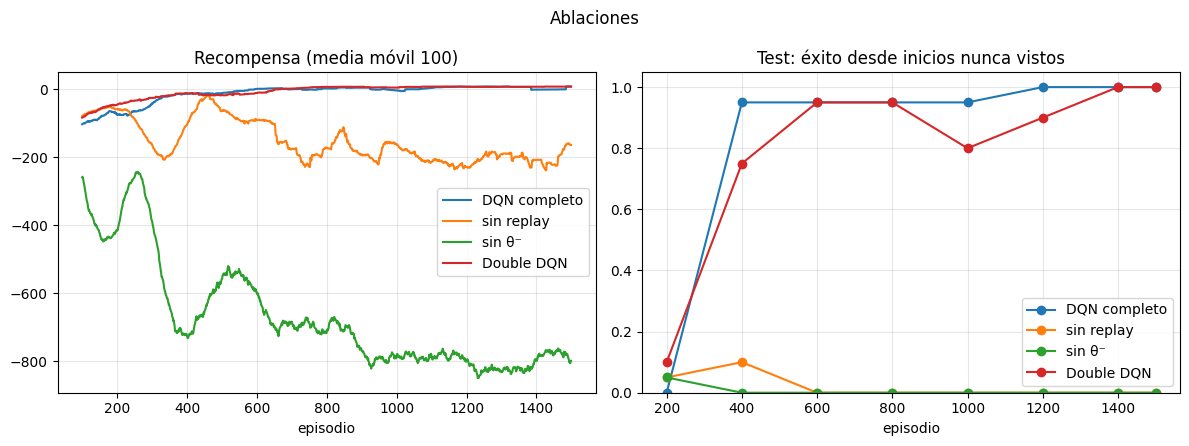
\includegraphics[width=\columnwidth]{figuras/05_ablaciones.png}
\caption{Ablaciones: DQN completo, sin \emph{replay}, sin red objetivo ($\theta^-$) y Double DQN.}
\label{fig:ablacion}
\end{figure}

\begin{table}[ht]
\caption{Ablaciones: tasa de éxito en el test}
\label{tab:ablacion}
\centering
\begin{tabular}{lc}
\toprule
Configuración & Éxito \\
\midrule
DQN completo        & 100\,\% \\
sin \emph{replay}   & 0\,\% \\
sin red objetivo ($\theta^-$) & 0\,\% \\
Double DQN          & 100\,\% \\
\bottomrule
\end{tabular}
\end{table}

\subsection{Transición estocástica}
\label{sec:estoc}
Se evalúa la robustez del agente frente a perturbaciones del entorno mediante la introducción de transiciones estocásticas (deslizamiento). Específicamente, se modela una probabilidad de deslizamiento proporcional a la pendiente local, bajo la cual la acción seleccionada es reemplazada por una dirección cardinal aleatoria. La Fig.~\ref{fig:estoc} compara el desempeño del agente en entornos deterministas frente a estocásticos. En ambas condiciones se alcanza el 100\,\% de éxito; no obstante, el entorno estocástico requiere una longitud media de trayectoria ligeramente mayor (102 pasos frente a 96). Estos resultados demuestran la adaptabilidad de la política ante incertidumbre de transición, una propiedad que la formulación clásica de Dijkstra no aborda.

\begin{figure}[ht]
\centering
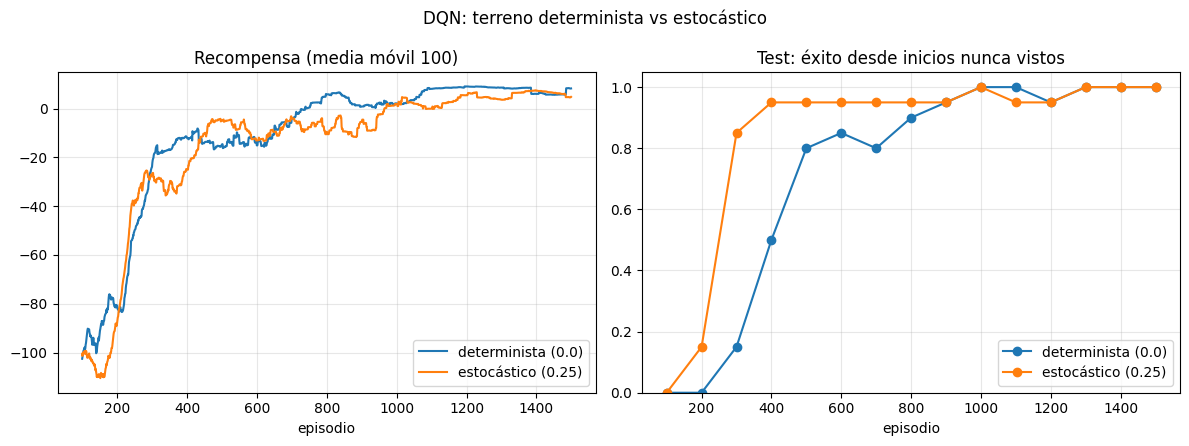
\includegraphics[width=\columnwidth]{figuras/06_estocastico.png}
\caption{DQN en terreno determinista vs estocástico (resbalón $0.25$).}
\label{fig:estoc}
\end{figure}

\subsection{Valor vs política: DQN y REINFORCE}
La comparación de desempeño entre el enfoque basado en valor (DQN) y el basado en política (REINFORCE) se presenta en la Fig.~\ref{fig:reinforce}. Ambos paradigmas alcanzan tasas de éxito elevadas (DQN: 100\,\%, REINFORCE: 95\,\%). Sin embargo, la dinámica de aprendizaje presenta diferencias sustanciales: DQN converge de forma suave y estable debido al efecto del búfer de reproducción y la red objetivo, mientras que REINFORCE exhibe una varianza significativa, con oscilaciones marcadas en el retorno episódico. Esta divergencia ilustra las características clásicas asociadas a cada familia de algoritmos.

\begin{figure}[ht]
\centering
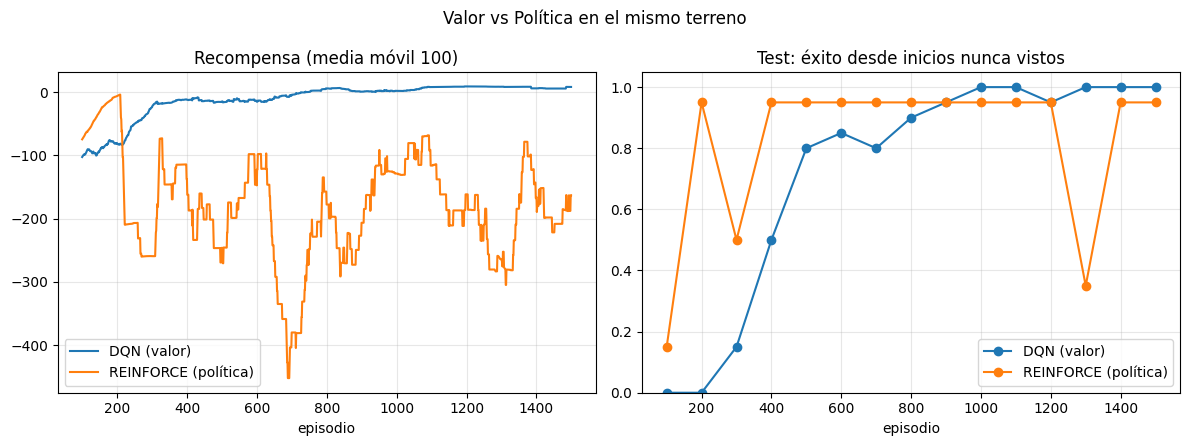
\includegraphics[width=\columnwidth]{figuras/07_dqn_vs_reinforce.png}
\caption{Valor vs política: DQN y REINFORCE en el mismo terreno.}
\label{fig:reinforce}
\end{figure}

\subsection{Divergencia con meta aleatoria}
La Fig.~\ref{fig:diverge} presenta el rendimiento de DQN ante la introducción de objetivos variables en cada episodio (configuración *goal-conditioned*). Se observa que la magnitud media de los valores $Q$ se mantiene estable hasta el episodio 1000, momento a partir del cual experimenta una divergencia asintótica, escalando de un valor de $\sim 1$ a más de $2400$. De forma simultánea, la tasa de éxito colapsa por debajo del 10\,\%. Esta inestabilidad se atribuye al sesgo de sobreestimación del operador de maximización acumulado mediante *bootstrapping*, justificando la adopción de un esquema de meta fija en el presente estudio.

\begin{figure}[ht]
\centering
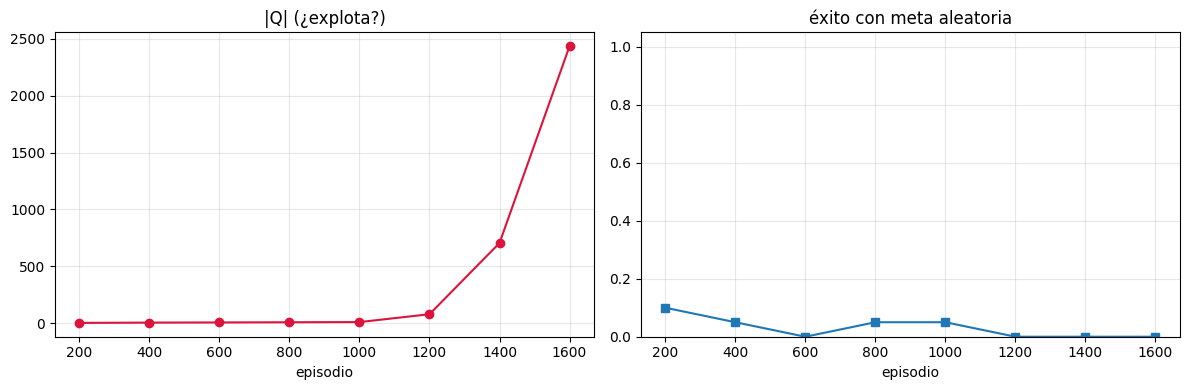
\includegraphics[width=\columnwidth]{figuras/08_divergencia.png}
\caption{Con meta aleatoria, la magnitud media de $Q$ (izq.) crece sin control (divergencia) y el éxito (der.) no se sostiene.}
\label{fig:diverge}
\end{figure}